\documentclass[a4paper,12pt,oneside]{book}

%-------------------------------Start of the Preable------------------------------------------------
\usepackage[english]{babel}
\usepackage{blindtext}
%packagr for hyperlinks
\usepackage{hyperref}
\hypersetup{
    colorlinks=true,
    linkcolor=blue,
    filecolor=magenta,
    urlcolor=cyan,
}

\urlstyle{same}
%use of package fancy header
\usepackage{fancyhdr}
\setlength\headheight{26pt}
\fancyhf{}
%\rhead{
\includegraphics[width=1cm]{logo}}
\lhead{\rightmark}
\rhead{
\includegraphics[width=1cm]{logo}}
\fancyfoot[RE, RO]{\thepage}
\fancyfoot[CE,CO]{\href{http://www.e-yantra.org}{www.e-yantra.org}}

\pagestyle{fancy}

%use of package for section title formatting
\usepackage{titlesec}
\titleformat{\chapter}
  {\Large\bfseries} % format
  {}                % label
  {0pt}             % sep
  {\huge}           % before-code

%use of package tcolorbox for colorful textbox
\usepackage[most]{tcolorbox}
\tcbset{colback=cyan!5!white,colframe=cyan!75!black,halign title = flush center}

\newtcolorbox{mybox}[1]{colback=cyan!5!white,
colframe=cyan!75!black,fonttitle=\bfseries,
title=\textbf{\Large{#1}}}

%use of package marginnote for notes in margin
\usepackage{marginnote}

%use of packgage watermark for pages
%\usepackage{draftwatermark}
%\SetWatermarkText{
\includegraphics{logo}}
\usepackage[scale=2,opacity=0.1,angle=0]{background}
\backgroundsetup{
contents={
\includegraphics{logo}}
}

%use of newcommand for keywords color
\usepackage{xcolor}
\newcommand{\keyword}[1]{\textcolor{red}{\textbf{#1}}}

%package for inserting pictures
\usepackage{graphicx}

%package for highlighting
\usepackage{color,soul}

%new command for table
\newcommand{\head}[1]{\textnormal{\textbf{#1}}}


%----------------------End of the Preamble---------------------------------------


\begin{document}

%---------------------Title Page------------------------------------------------
\begin{titlepage}
\raggedright
{\Large eYSIP2016\\[1cm]}
{\Huge\scshape Robot State Collector\\[.1in]}
\vfill
\begin{flushright}
{\large Amanpreet Singh \\}
{\large Amit Raushan \\}
{\large Shubham Gupta \\}
{\large Duration of Internship: $ 10/06/2016-24/07/2016 $ \\}
\end{flushright}

{\itshape 2016, e-Yantra Publication}

\end{titlepage}

\tableofcontents

%------------------------------------------------------------------------

\chapter[Robot State Collector]{Robot State Collector}
\section{Abstract}

\hspace{5mm}This project aims at developing a State Collection Algorithm which is easy to integrate with user code without interfering with it. Our code should be capable of collecting the sensor values periodically. It should also send this data to the GUI developed for this specific purpose. The GUI should be able to encrypt the collected data and send it to the e-Yantra servers.

This would be helpful in virtually re-creating runs ,using the user's code and the data collected by the State Collection Algorithm.

The main tasks involved in the project are :

\begin{enumerate}

    \item Collecting timed data about the state of the robot(sensors etc.).
    \item Developing a GUI that picks up the data from the robot, encrypts it and send it to e-yantra servers.
    \item Writing server side code to receive and decrypt the state information obtained from GUI developed in step 2.

\end{enumerate}
\newpage

\section{Completion Status}

\begin{enumerate}

    \item Successfully collected the data on Fire Bird V and Tiva Robot using the State Collection Algorithm.
    \item To avoid storing the data on the volatile memory on any robot a XBee module is used which directly sends the data to the GUI wirelessly. This also saves space on the robot's memory.
    \item Developed a GUI to read the incoming data from the Robot. The GUI encrypts the data and sends it back to the server. The GUI is also capable of detecting if any changes were made to the file before sending it to the server.
    \item Implemented a Demo Server.
    \item Made a Robot using the Tiva board so as to check that our algorithm and GUI are not restricted to only Fire Bird V.
    \item Performed state collection on the newly developed robot.
\newpage

\end{enumerate}

\section{Hardware Parts Used}

\begin{itemize}
  \item Hardware used with Fire Bird V :
  \\
  \begin{figure}[h]
        \centering
        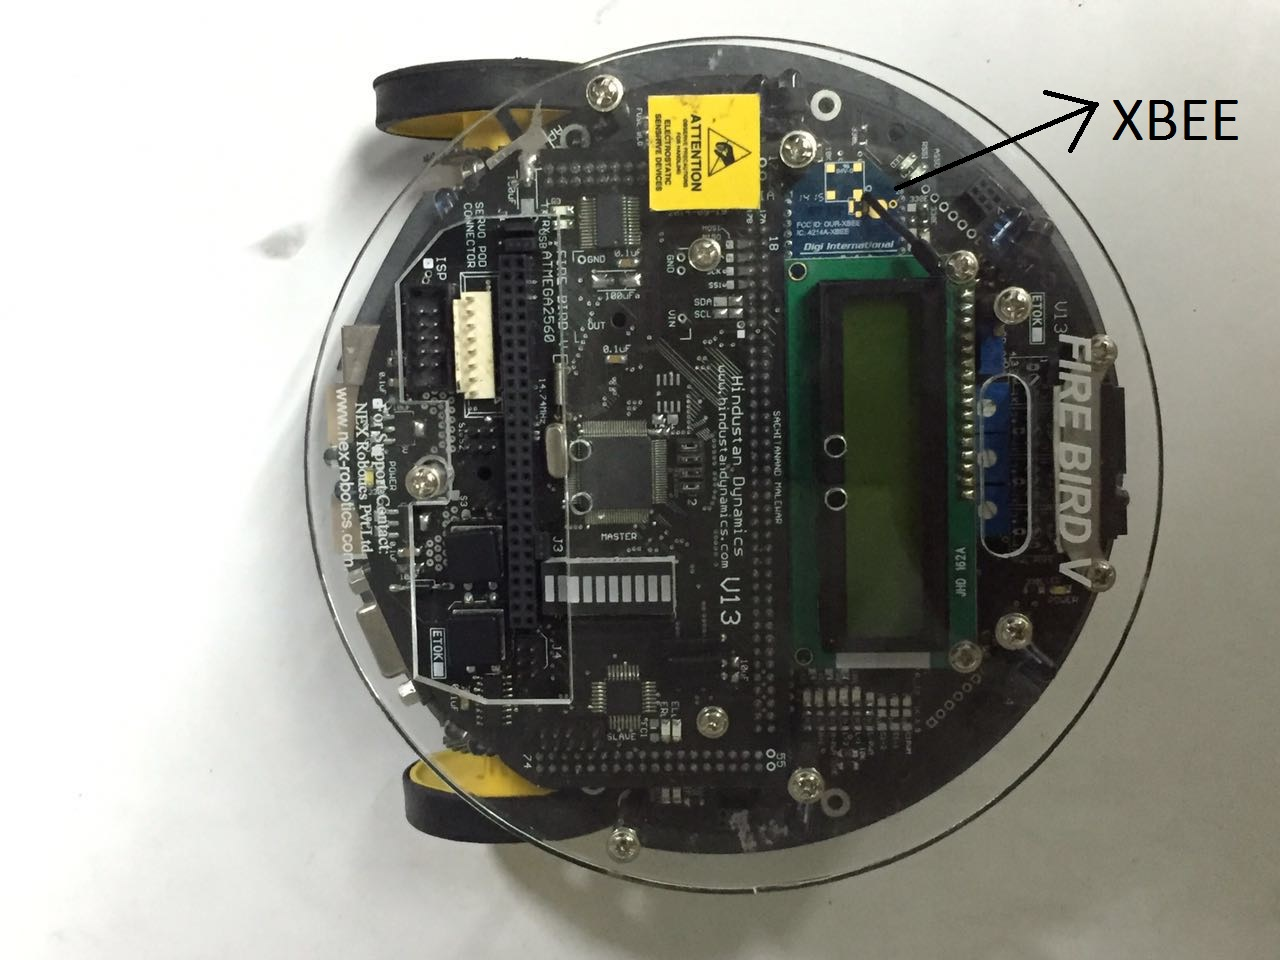
\includegraphics[scale=0.2]{firebird_V}
        \caption{Fire Bird V with XBee module}
      \end{figure}

  \begin{enumerate}
    \item XBee Module.\\
    \href{https://www.sparkfun.com/datasheets/Wireless/Zigbee/XBee-Datasheet.pdf}{ Datasheet}
    \begin{figure}[h]
        \centering
        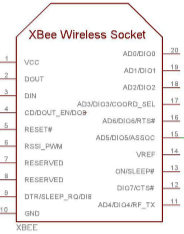
\includegraphics[scale=0.35]{XBee.jpg}
        \caption{XBee module}
      \end{figure}
      \newpage
    \item XBee Module and adapter to receive data on a Laptop/PC.\par

    \begin{figure}[!ht]
        \centering
        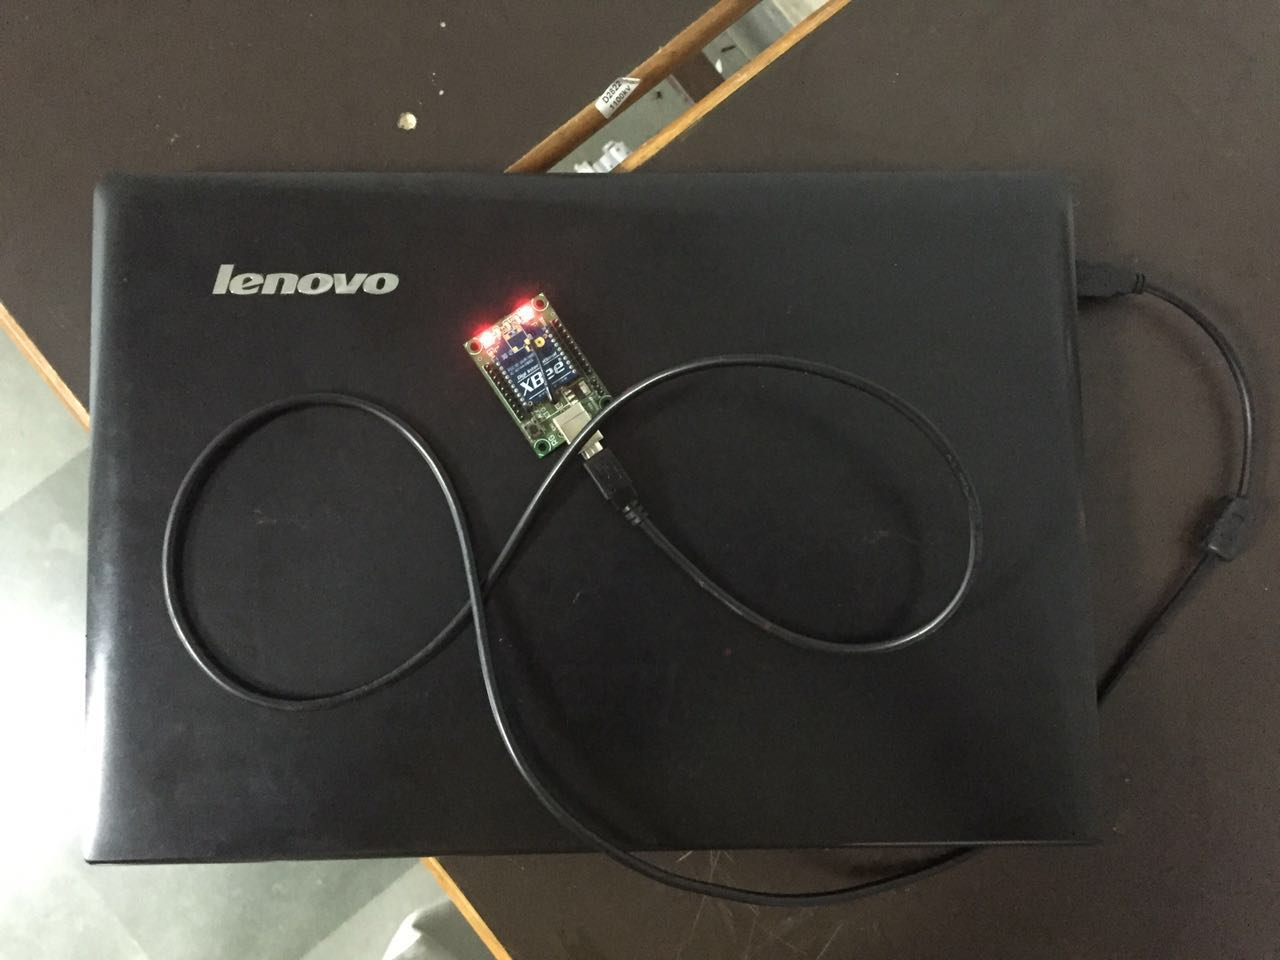
\includegraphics[scale=0.15]{adapter_board}
        \caption{XBee with adapter connected to laptop}
      \end{figure}
  \end{enumerate}

  \item Hardware used to build a Robot using Tiva board (TM4C123GXL)\\
  \href{http://www.ti.com.cn/cn/lit/ds/symlink/tm4c123gh6pm.pdf}{ Datasheet}\\
  \href{http://www.ti.com/lit/ug/spmu298a/spmu298a.pdff}{ Pheripheral Driver Library}\\
  \href{http://www.mouser.com/ds/2/405/spmu296-242111.pdf}{User's Guide}
  \begin{figure}[h]
        \centering
        \includegraphics[scale=0.2]{Tiva}
        \caption{Tiva C Series TM4C123G LaunchPad}
      \end{figure}
       \newpage
  \begin{enumerate}
   \item 2x DG02S Mini DC Gear motor.\\
   \href{http://cdn.sparkfun.com/datasheets/Robotics/DG02S.pdf}{ Datasheet}
   \begin{figure}[!ht]
        \centering
        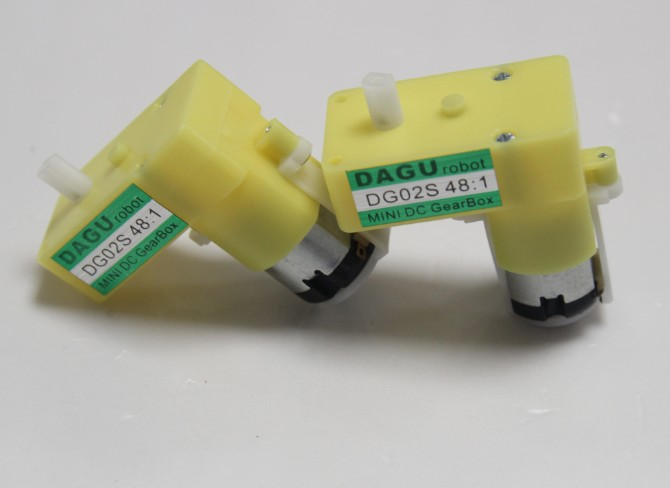
\includegraphics[scale=0.25]{motor}
        \caption{DC Geared motor}
      \end{figure}

    \item 2x Wheel - 65mm in Diameter.
    \begin{figure}[h]
        \centering
        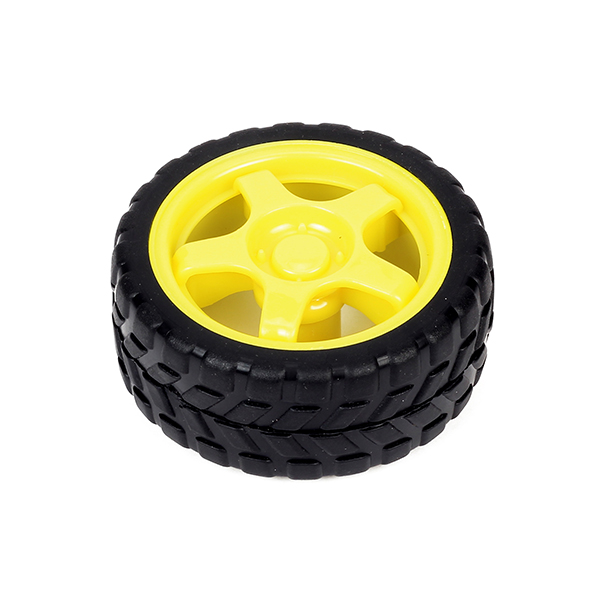
\includegraphics[scale=0.22]{wheel}
        \caption{Wheel}
      \end{figure}
    \item L293D - Motor Driver.\\
    \href{http://www.engineersgarage.com/sites/default/files/L293D.pdf}{ Datasheet}\par
   \begin{figure}[!ht]
        \centering
        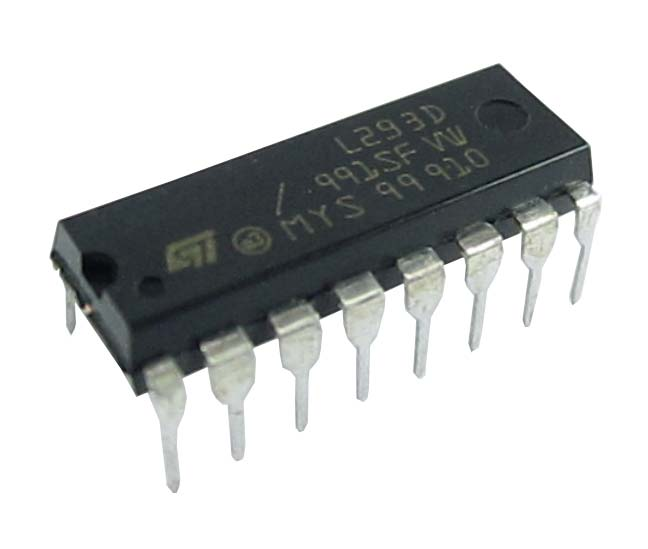
\includegraphics[scale=0.2]{l293d}
        \caption{Motor Driver IC}
      \end{figure}
      \newpage
    \item 16x2 LCD.\\
    \href{http://www.engineersgarage.com/sites/default/files/LCD\%2016x2.pdf}{ Datasheet}\par
   \begin{figure}[!ht]
        \centering
        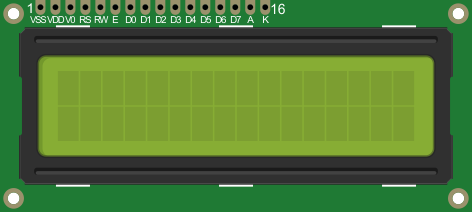
\includegraphics[scale=0.85]{lcd}
        \caption{LCD 16x2 Display}
      \end{figure}
    \item White Line Sensor Module.\\
    \href{http://www.nex-robotics.com/images/downloads/3\%20channel\%20line\%20sensor.pdf}{ Manual}\par
   \begin{figure}[!ht]
        \centering
        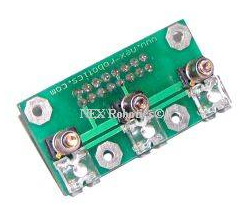
\includegraphics[scale=0.85]{whiteline}
        \caption{3 Channel Whiteline Sensors}
      \end{figure}
    \item Sharp 0A41SK sensor.\\
    \href{http://www.Sharp-world.com/products/device/lineup/data/pdf/datasheet/gp2y0a41sk_e.pdf}{ Datasheet}\par
   \begin{figure}[!ht]
        \centering
        \includegraphics[scale=0.8]{Sharp}
        \caption{Sharp Sensor}
      \end{figure}
    \item Caster Wheel.
    \begin{figure}[!ht]
        \centering
        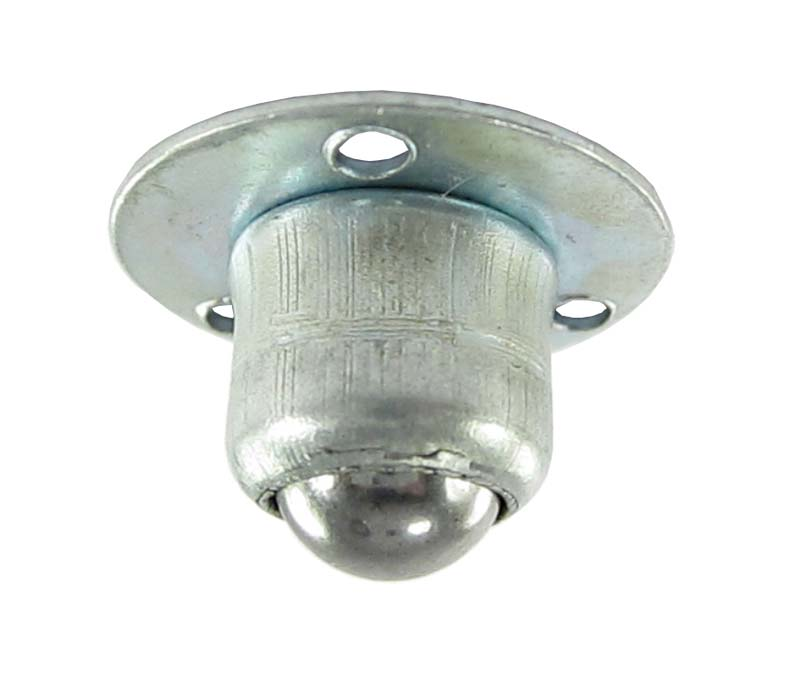
\includegraphics[scale=0.15]{caster}
        \caption{Caster Wheel}
      \end{figure}
    \item LM3237 - Voltage Regulator.\\
    \href{http://pdf.datasheetarchive.com/indexerfiles/Datasheet-044/DSA0017815.pdf}{ Datasheet}\par
   \begin{figure}[!ht]
        \centering
        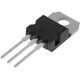
\includegraphics[scale=1]{lm}
        \caption{LM3237}
      \end{figure}
    \item Heat Sink.
    \begin{figure}[!ht]
        \centering
        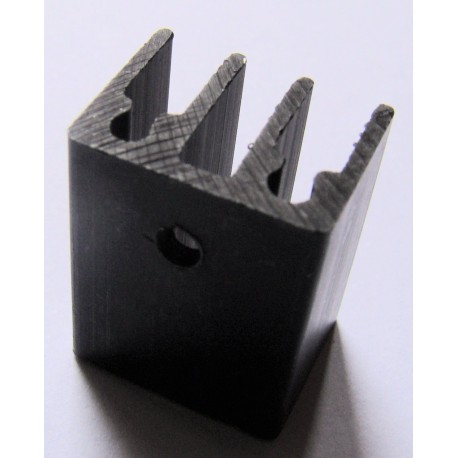
\includegraphics[scale=0.25]{heat}
        \caption{Heat Sink}
      \end{figure}
      \newpage
    \item 10uF Electrolyte Capacitor.
    \begin{figure}[!ht]
        \centering
        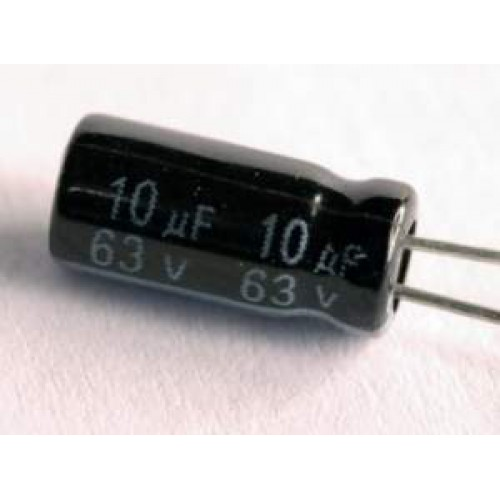
\includegraphics[scale=0.35]{cap}
        \caption{Capacitor}
      \end{figure}
    \item Multi-purpose PCB board. \\
    \begin{figure}[!h]
        \centering
        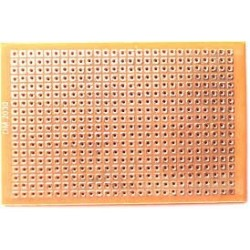
\includegraphics[scale=0.6]{pcb}
        \caption{PCB Board}
      \end{figure}
\newpage
    \item 12V Rechargeable Battery.
    \begin{figure}[!h]
        \centering
        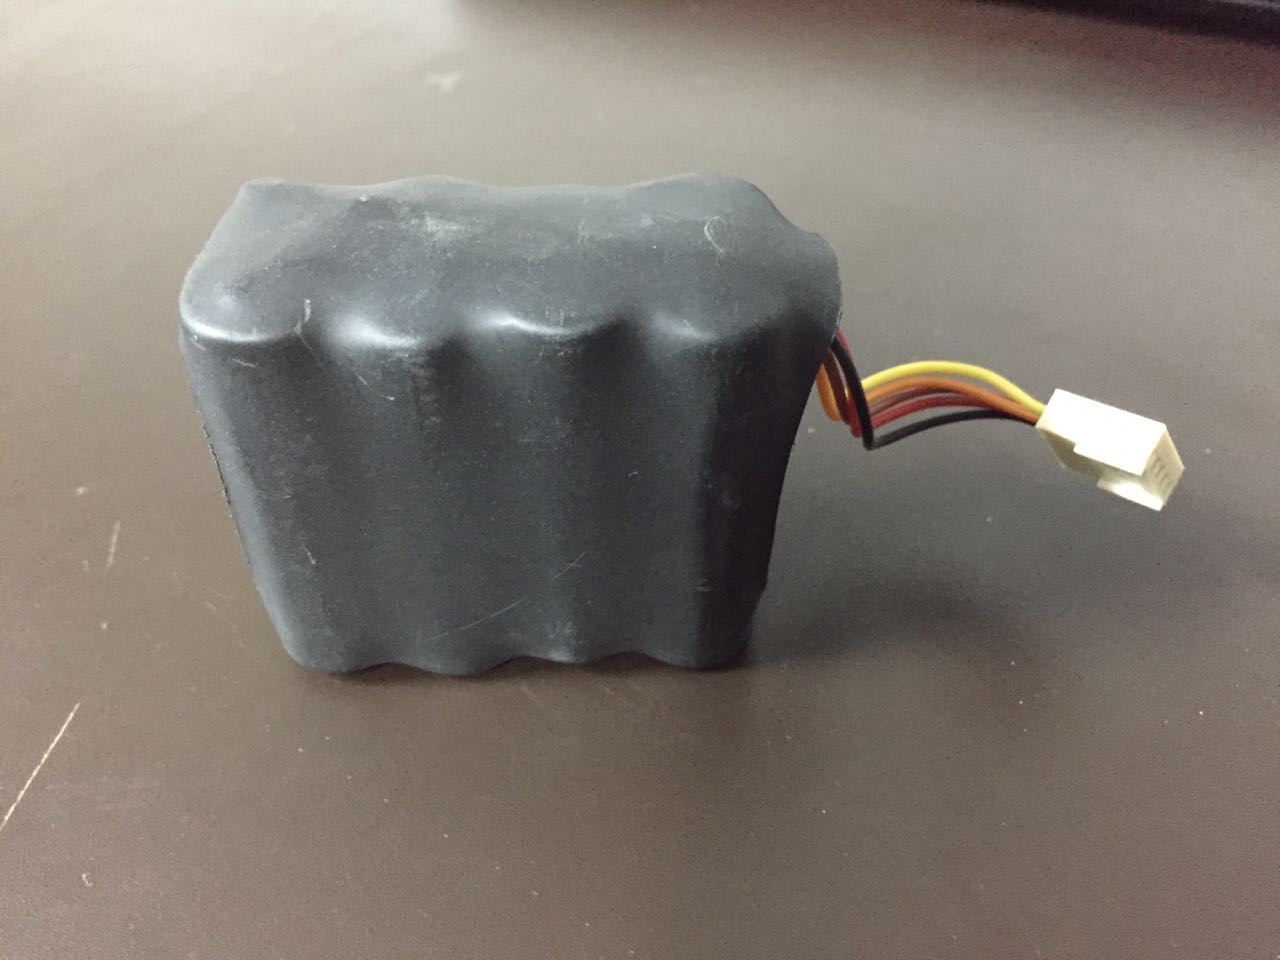
\includegraphics[scale=0.12]{battery}
        \caption{12V Rechargeable Battery}
      \end{figure}
    \item 20 Pin Planar Cable.
    \begin{figure}[!h]
        \centering
        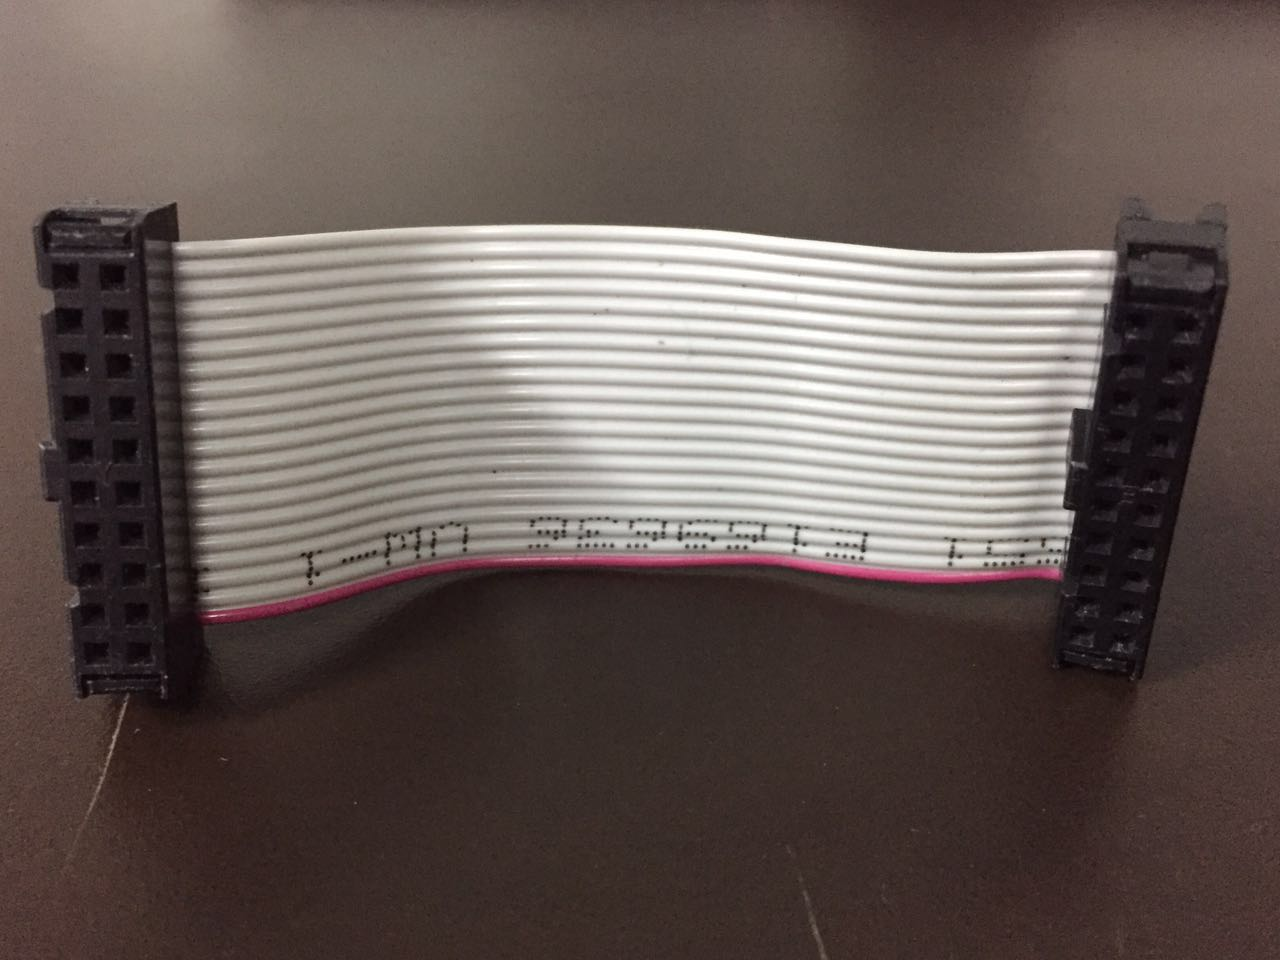
\includegraphics[scale=0.1]{wire}
        \caption{20 Pin Connector Wire}
      \end{figure}
    \item Female Bug Strip.
    \\
    \begin{figure}[!h]
        \centering
        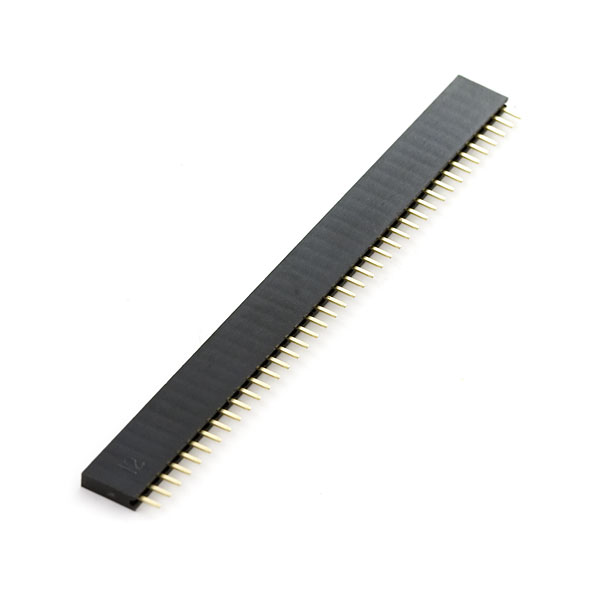
\includegraphics[scale=0.25]{fmbug}
        \caption{Female Bug Strip}
      \end{figure}
      \newpage
    \item Male Bug Strip.
    \begin{figure}[!h]
        \centering
        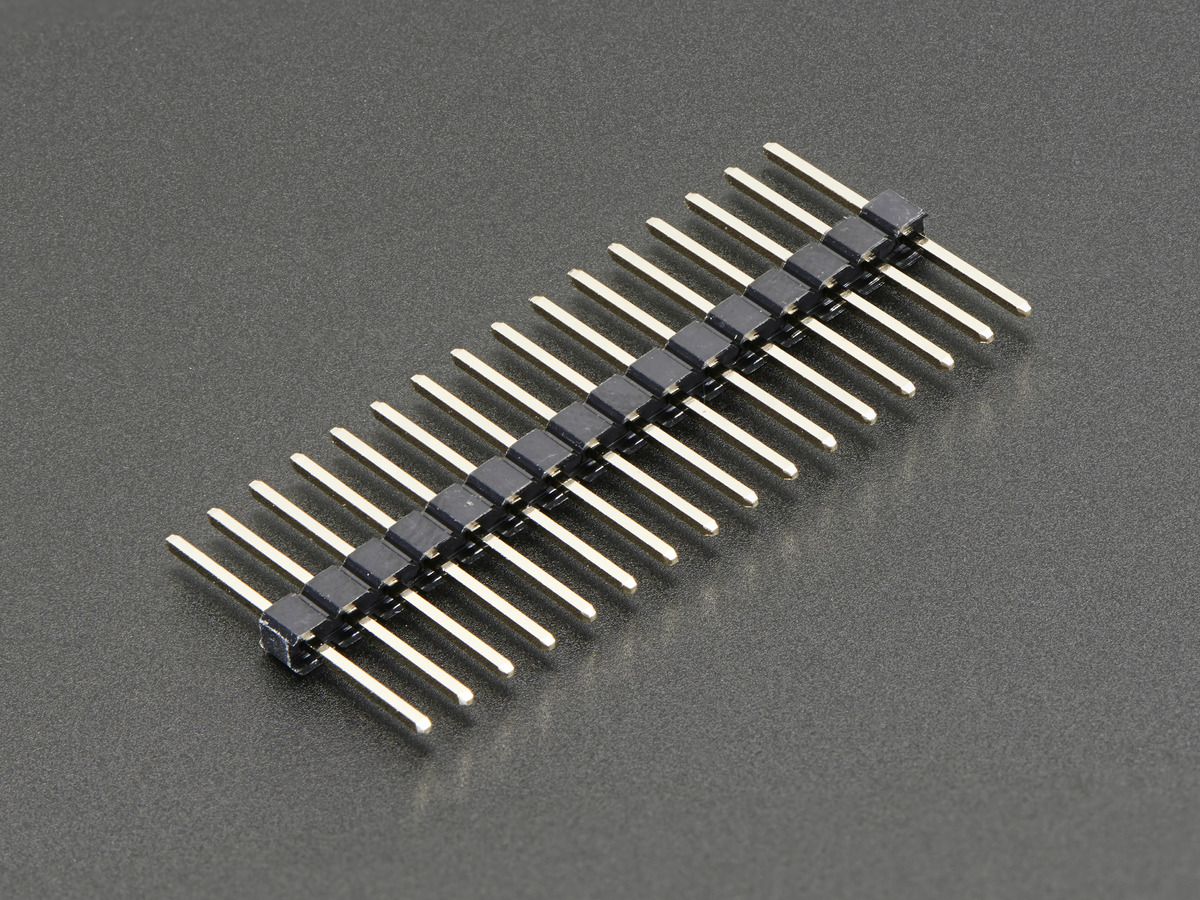
\includegraphics[scale=0.12]{mbug}
        \caption{Male Bug Strip}
      \end{figure}
    \item Male to Female Jumper Wires.
    \begin{figure}[!h]
        \centering
        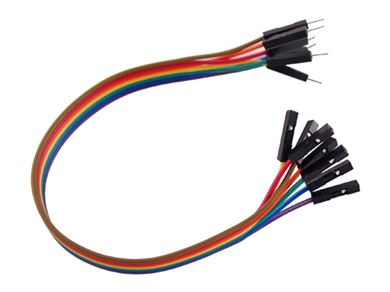
\includegraphics[scale=0.45]{jumper}
        \caption{Jumper Wires}
      \end{figure}\\
    \item Plastic Chassis.\\
     \par
    \begin{figure}[!h]
        \centering
        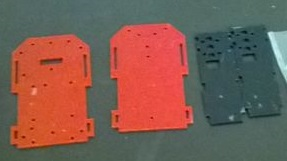
\includegraphics[scale=0.75]{chasis}
        \caption{Chassis}
      \end{figure}
      \newpage
  \end{enumerate}

\end{itemize}
\newpage
\section{Software Used}
\begin{itemize}
  \item Atmel Studio 6.0\\
  \href{http://www.atmel.com/forms/software-download.aspx?target=tcm:26-41305}{ Download link}
  \item XCTU-NG\\
  \href{http://www.digi.com/products/XBee-rf-solutions/xctu-software/xctu}{ Download link}
  \item Serial Terminal\\
  \href{http://www.nex-robotics.com/images/downloads/Terminal\%20Setup.zip}{Download link}
  \item Code Composer Studio v6.1.3\\
  \href{http://www.ti.com/tool/ccstudio}{Download link}


  \item NetBeans IDE 8.1\\
  \href{https://netbeans.org/downloads/}{Download link}
  \item AVR Bootloader\\
  \href{http://www.nex-robotics.com/images/downloads/AVR\%20Boot\%20Loader.zip}{Download link}
\end{itemize}
\newpage
\section{Assembly of Hardware}
\subsection{Fire Bird V Robot}
XBee module is attached with Fire Bird V Robot to transmit the collected state information.
\begin{figure}[h]
        \centering
        \includegraphics[scale=0.19]{XBee_connected}
        \caption{XBee connected with Fire Bird V}
      \end{figure}
\subsection{Tiva Robot}

   \begin{figure}[h]
        \centering
        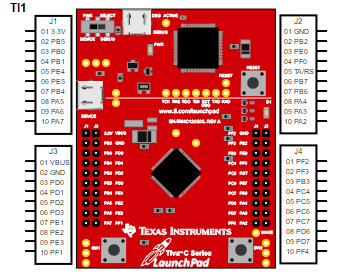
\includegraphics[scale=0.8]{Tiva_pin}
        \caption{Tiva Board Pin Location}
      \end{figure}

Connections of PORT pins of Tiva board with different components:\\
\begin {enumerate}
\item Interfacing of white line sensor
\begin{center}
	\begin{figure}[h]
		\centering
		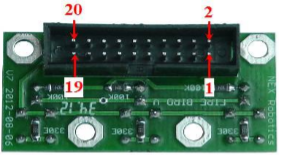
\includegraphics[scale=1]{whiteline_pin}
		\caption{Pin Configuration of White Line Sensor}
	\end{figure}

 \begin{tabular}{| c | c |}
 
 	\hline
 	\textbf{Tiva Port Pins} & \textbf{Sensors Pin}\\
 
 	\hline
 	PE1 & 1\\
 	\hline
 	PE2 & 3\\
 	\hline
 	PE3 & 5 \\
 	\hline
 		VCC & 2\\
 		\hline
 			VCC & 4 \\
 			\hline
 				VCC & 6 \\
 				\hline
 	GND & 15\\
 	\hline
 		GND & 16\\
 		\hline
 			GND & 17\\
 			\hline
 	VCC & 19 \\
 	\hline
 \end{tabular}
 \end{center}
\item Interfacing of Sharp sensor\\
\begin{center}
\begin{tabular}{| c | c |}
	\hline
	\textbf{Tiva Port Pins} & \textbf{Sensor Pins}\\
	\hline
	PE0 & SIGNAL\\
	\hline
	GND & GND\\
	\hline
	VCC & VCC \\
	\hline
\end{tabular}
\end{center}
\newpage
\item Interfacing of Motor Driver IC\\
	\begin{figure}[h]
		\centering
		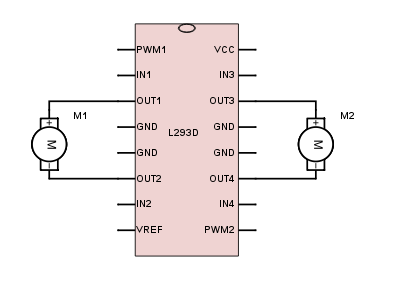
\includegraphics[scale=1]{MOTOR_DRIVER}
		\caption{Pin Configuration of Motor Driver IC}
	\end{figure}
	\begin{center}
\begin{tabular}{| c | c |}
	\hline
	\textbf{Tiva Port Pins} & \textbf{L293D Pins}\\
	\hline
	PE4 & PWM1\\
	\hline
	PA2 & INPUT1\\
	\hline
	PA3 & INPUT2 \\
	\hline
	GND & GND\\
	\hline
	VCC & VCC \\
	\hline
	PE5 & PWM2 \\
	\hline
	PA6 & INPUT3\\
	\hline
	PA7 & INPUT4 \\
	\hline
	VBUS & VREF \\
	\hline
\end{tabular}
\end{center}
\newpage
\item Interfacing of XBee module\\
\begin{figure}[h]
	\centering
	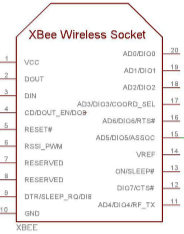
\includegraphics[scale=1]{XBee}
	\caption{Pin Configuration of XBee Socket}
\end{figure}
\begin{center}
\begin{tabular}{| c | c |}
	\hline
	\textbf{Tiva Port Pins} & \textbf{XBee Pins}\\
	\hline
	PC4 & DOUT\\
	\hline
	PC5 & DIN\\
	\hline
	GND & GND\\
	\hline
	VCC & VCC \\
	\hline
\end{tabular}
\end{center}
\item Interfacing of Buzzer
\begin{figure}[h]
	\centering
	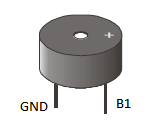
\includegraphics[scale=1]{speaker}
	\caption{Pin Configuration of Buzzer}
\end{figure}
\begin{center}
	\begin{tabular}{| c | c |}
		\hline
		\textbf{Tiva Port Pins} & \textbf{Buzzer Pins}\\
		\hline
		PF0 & B1\\
		\hline
		GND & GND\\
		\hline
	\end{tabular}
\end{center}
\newpage
\item Interfacing of LCD
\begin{figure}[h]
	\centering
	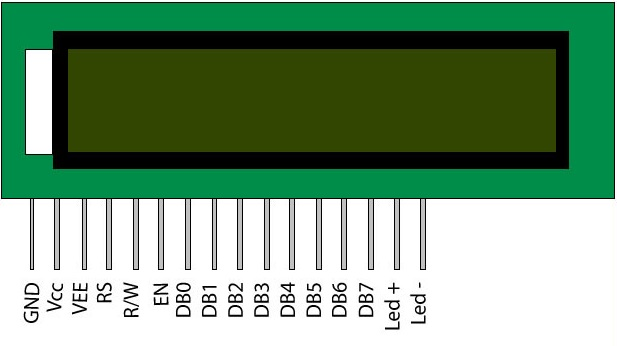
\includegraphics[scale=0.5]{lcd_pin}
	\caption{Pin Configuration of LCD Display}
\end{figure}
\begin{center}
	\begin{tabular}{| c | c |}
		\hline
		\textbf{Tiva Port Pins} & \textbf{LCD Pins}\\
		\hline
		GND & GND\\
		\hline
		VCC & Vcc\\
		\hline
		GND & VEE \\
		\hline
		PA4 & RS\\
		\hline
		PA5 & R/W \\
		\hline
		PC6 & EN \\
		\hline
		PB0 & DB0\\
		\hline
		PB1 & DB1 \\
		\hline
		PB2 & DB2\\
		\hline
		PB3 & DB3 \\
		\hline
		PB4 & DB4 \\
		\hline
		PB5 & DB5 \\
		\hline
		PB6 & DB6 \\
		\hline
		PB7 & DB7 \\
		\hline
			VCC & Led+ \\
			\hline
				GND & Led- \\
				\hline
	\end{tabular}
\end{center}
\end{enumerate}
\newpage
\subsection*{Block Diagram}
Basic connections of different components used with Tiva Robot.
\\
\begin{figure}[h]
        \centering
        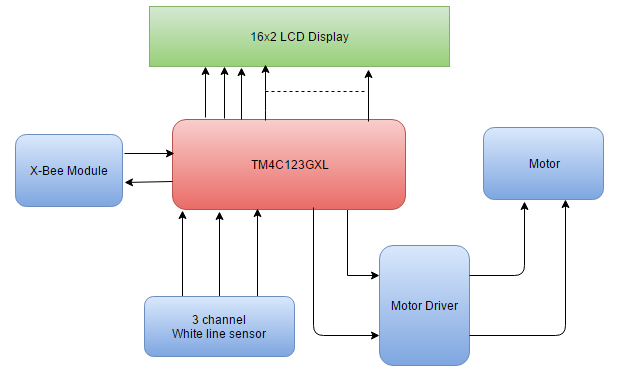
\includegraphics[scale=0.7]{Block}
        \caption{Block Diagram of Tiva Robot}
      \end{figure}
\subsection*{Voltage Regulator Circuit Diagram}
\begin{figure}[h]
	\centering
	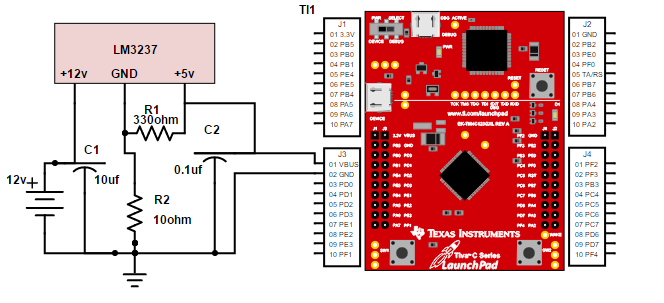
\includegraphics[scale=0.7]{Voltage_Regulator_Circuit}
	\caption{Circuit Diagram of Voltage Regulator Circuit}
\end{figure}

      \newpage
\subsection{Steps for Assembling Tiva Robot}
\begin{enumerate}
\item Gather/Buy all the components to be used for building the Robot.
\begin{figure}[h]
        \centering
        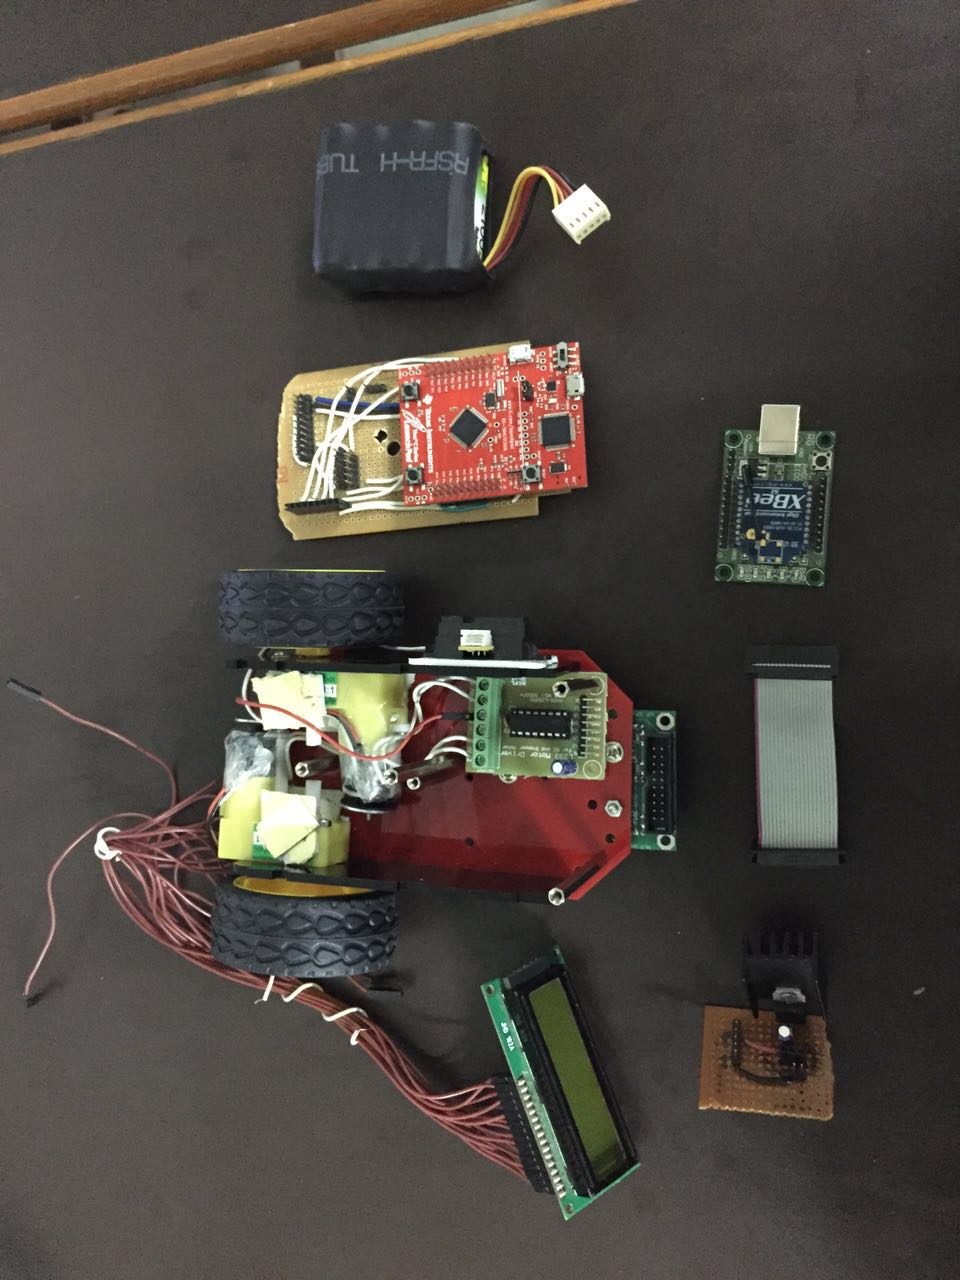
\includegraphics[scale=0.16]{all_components}
        \caption{All the components used to build the Robot.}
      \end{figure}
\item Assemble the chassis, two DC geared motors and two wheels. Then connect the motors with the Motor Driver IC.
\begin{figure}[h]
        \centering
        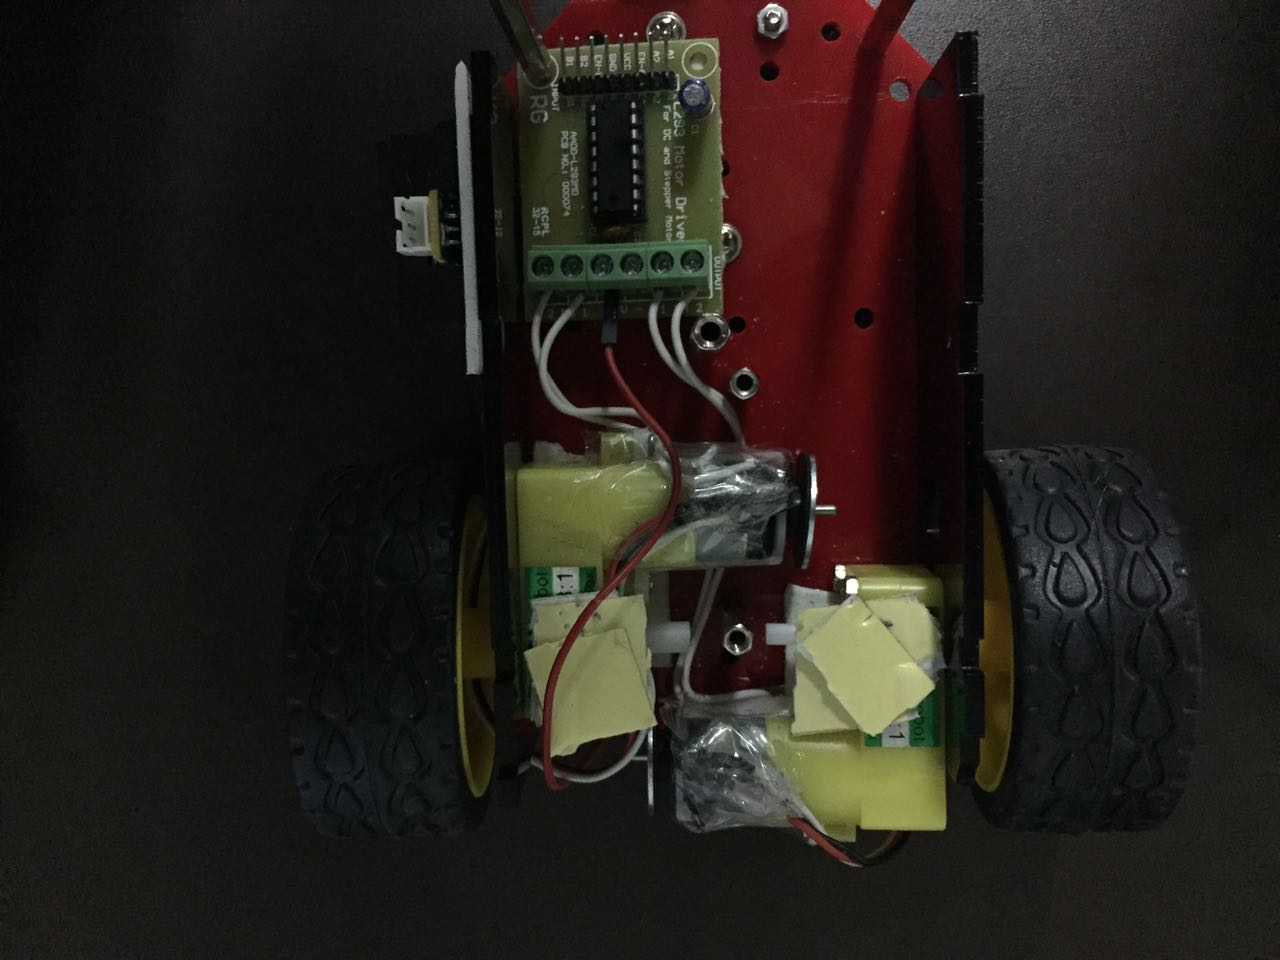
\includegraphics[scale=0.16]{motor_2_ic}
        \caption{Motors and wheels attached to chassis}
      \end{figure}
      \newpage
\item Connect the White Line sensors and Caster wheel to the chassis.
\begin{figure}[h]
        \centering
        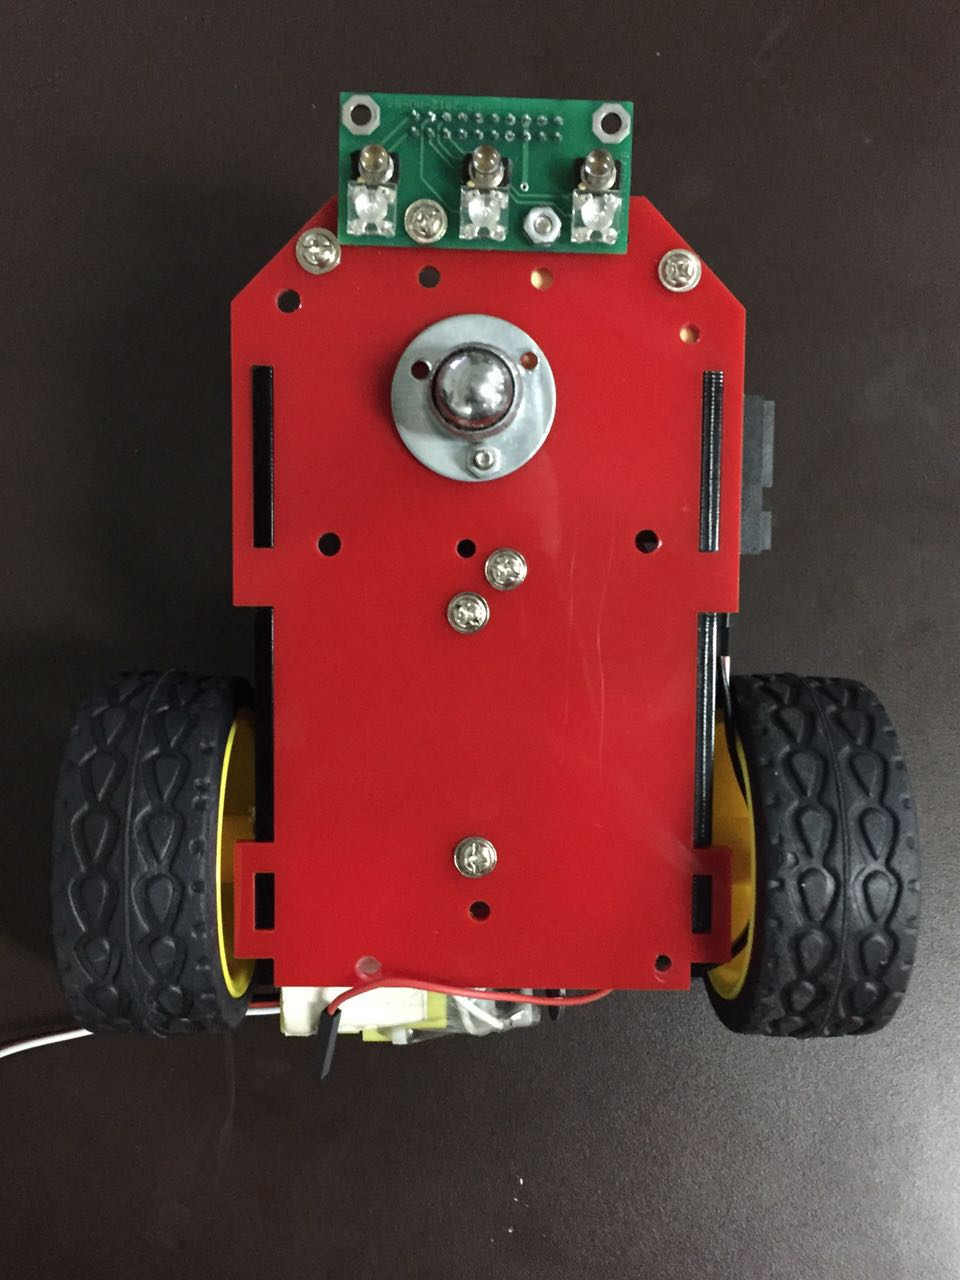
\includegraphics[scale=0.16]{caster_whiteline}
        \caption{Caster Wheel and White Line Sensors attached to chassis}
      \end{figure}

\item Attach Sharp Sensor to the chassis.
\begin{figure}[h]
        \centering
        \includegraphics[scale=0.16]{a_Sharp}
        \caption{Sharp Sensor attached to chassis}
      \end{figure}
      \newpage

\item Attach the Buzzer to the PCB board. Using the male bug strips (4x10) desgin a PCB board to which the Tiva board will be attached.
\begin{figure}[h]
        \centering
        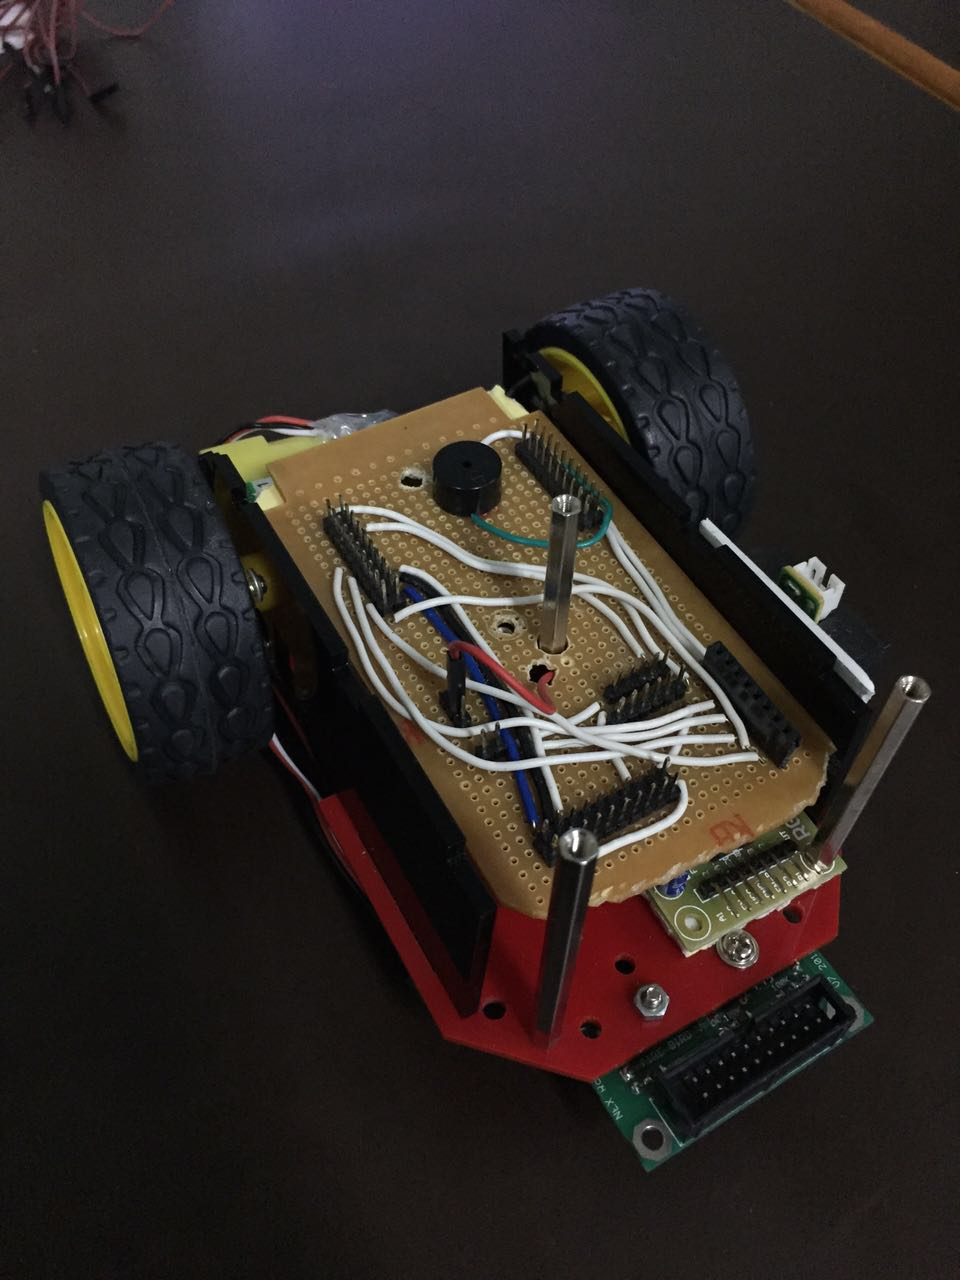
\includegraphics[scale=0.16]{buzzer}
        \caption{Buzzer which would be beneath the Tiva board}
      \end{figure}
\item Attach Tiva board (TM4C123GXL) on the PCB board.
\begin{figure}[h]
        \centering
        \includegraphics[scale=0.13]{Tiva_attatched}
        \caption{Tiva board fitted}
      \end{figure}
    \newpage

\item Connect White Line Sensors using the 20 pin connector.
\begin{figure}[h]
        \centering
        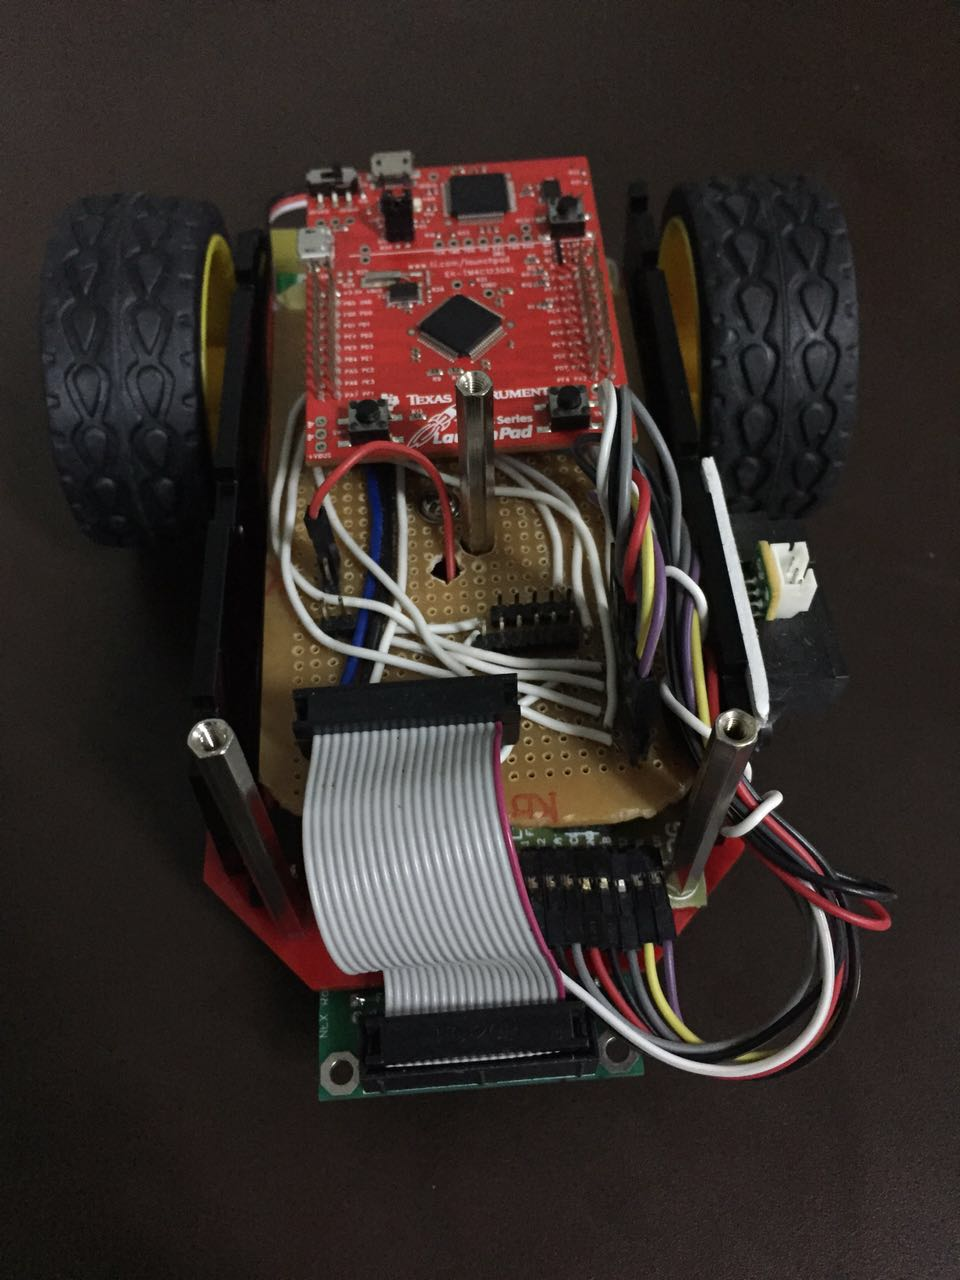
\includegraphics[scale=0.16]{wh_attatched}
        \caption{Whiteline Sensors are now connected to the Tiva board.}
      \end{figure}

\item Connect Sharp Sensor and Motor Driver IC to the Tiva board.
\begin{figure}[h]
        \centering
        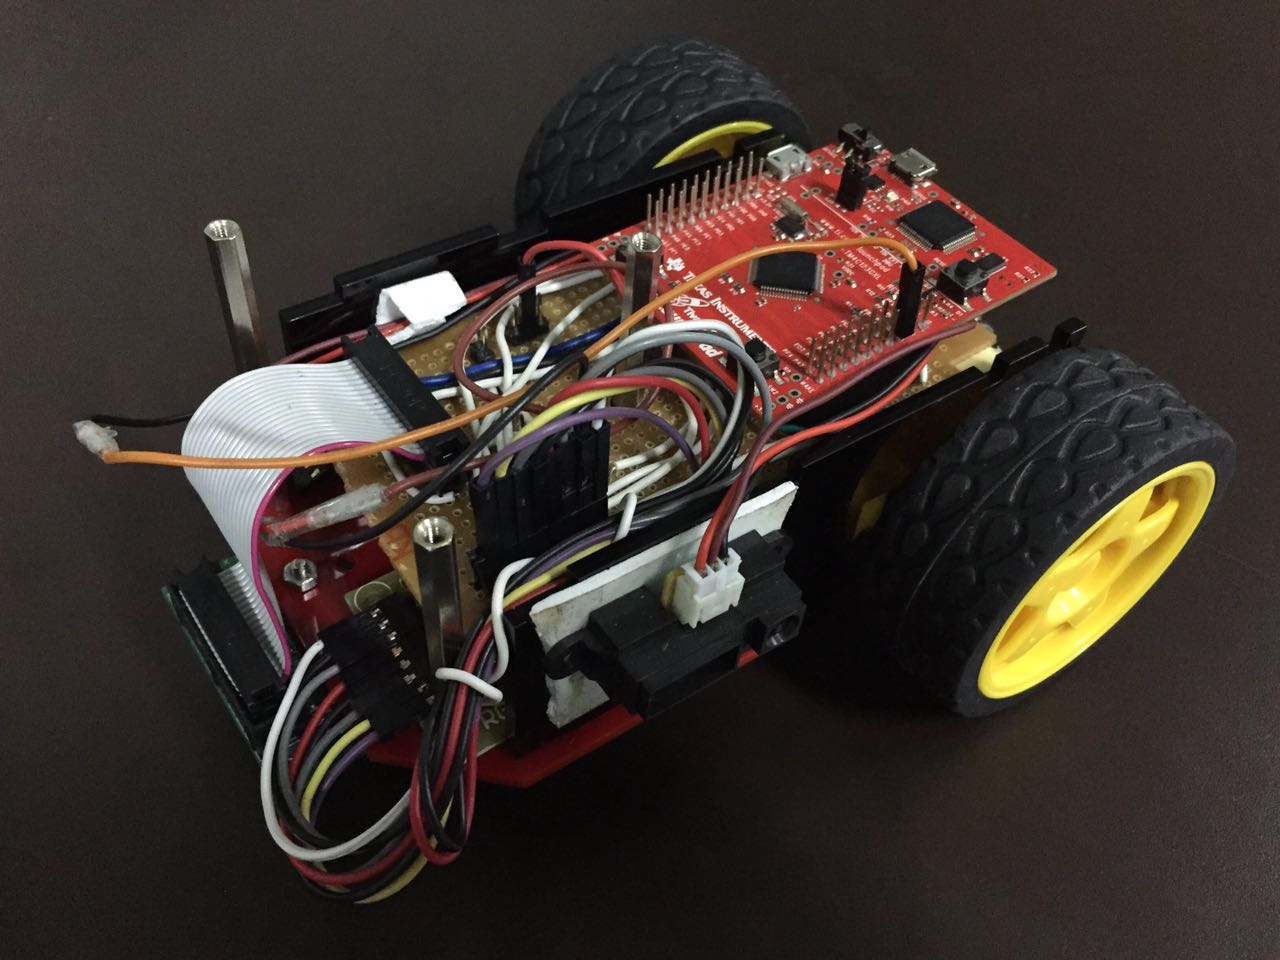
\includegraphics[scale=0.16]{all_connected}
        \caption{Sharp Sensor and Motor Driver IC are now connected to the Tiva board.}
      \end{figure}
      \newpage

\item Connect the LCD to the Tiva board.
\begin{figure}[h]
        \centering
        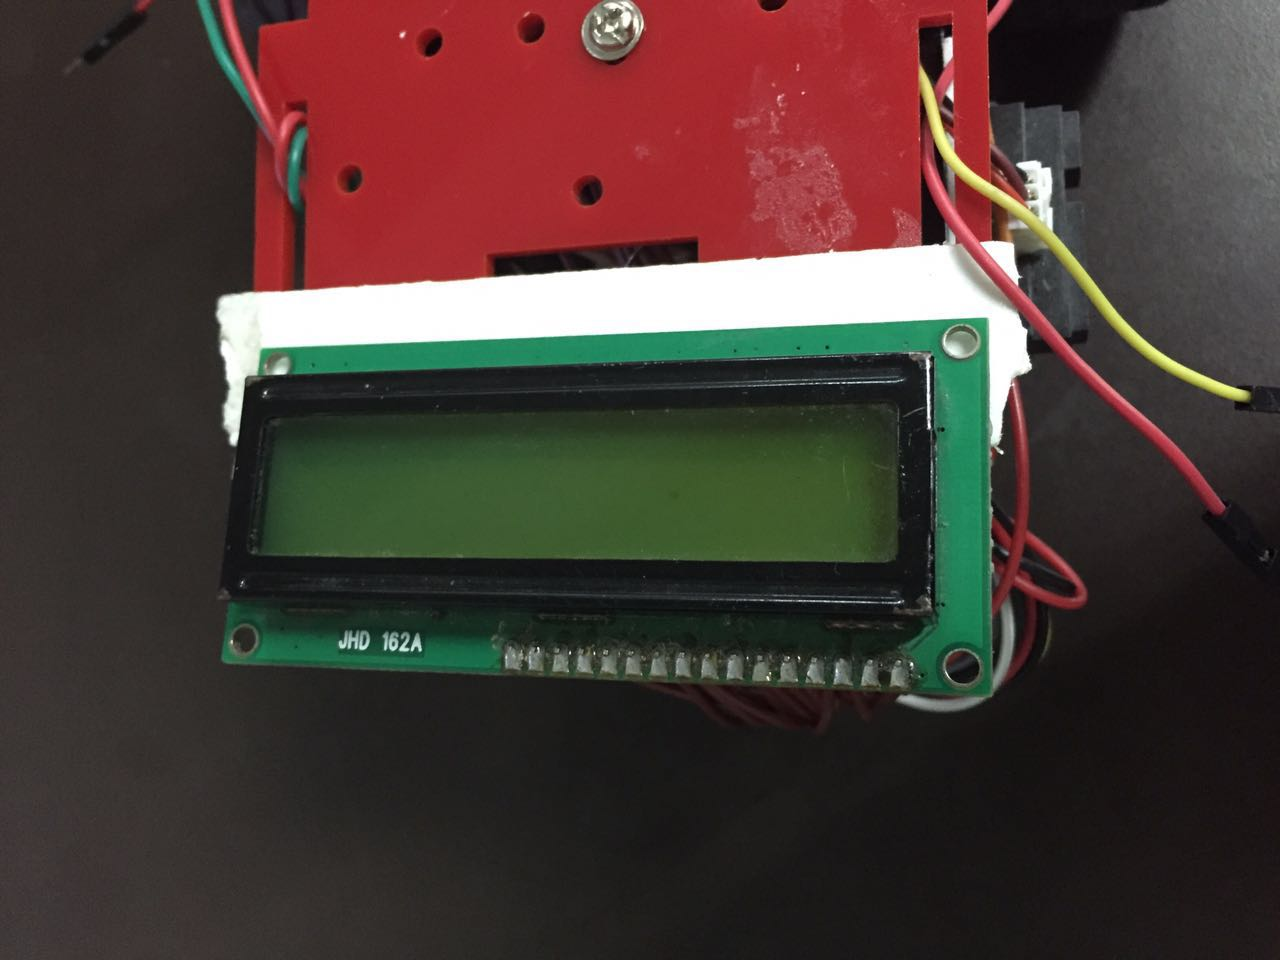
\includegraphics[scale=0.16]{lcd_a}
        \caption{LCD after being attached to the Robot.}
      \end{figure}

\item Connect the XBee to the Tiva board.
\begin{figure}[h]
        \centering
        \includegraphics[scale=0.16]{XBee_a}
        \caption{XBee after being attached to the Robot.}
      \end{figure}
      \newpage

\item Connect the Voltage Regulator Circuit and Battery to the Tiva board.
\begin{figure}[h]
        \centering
        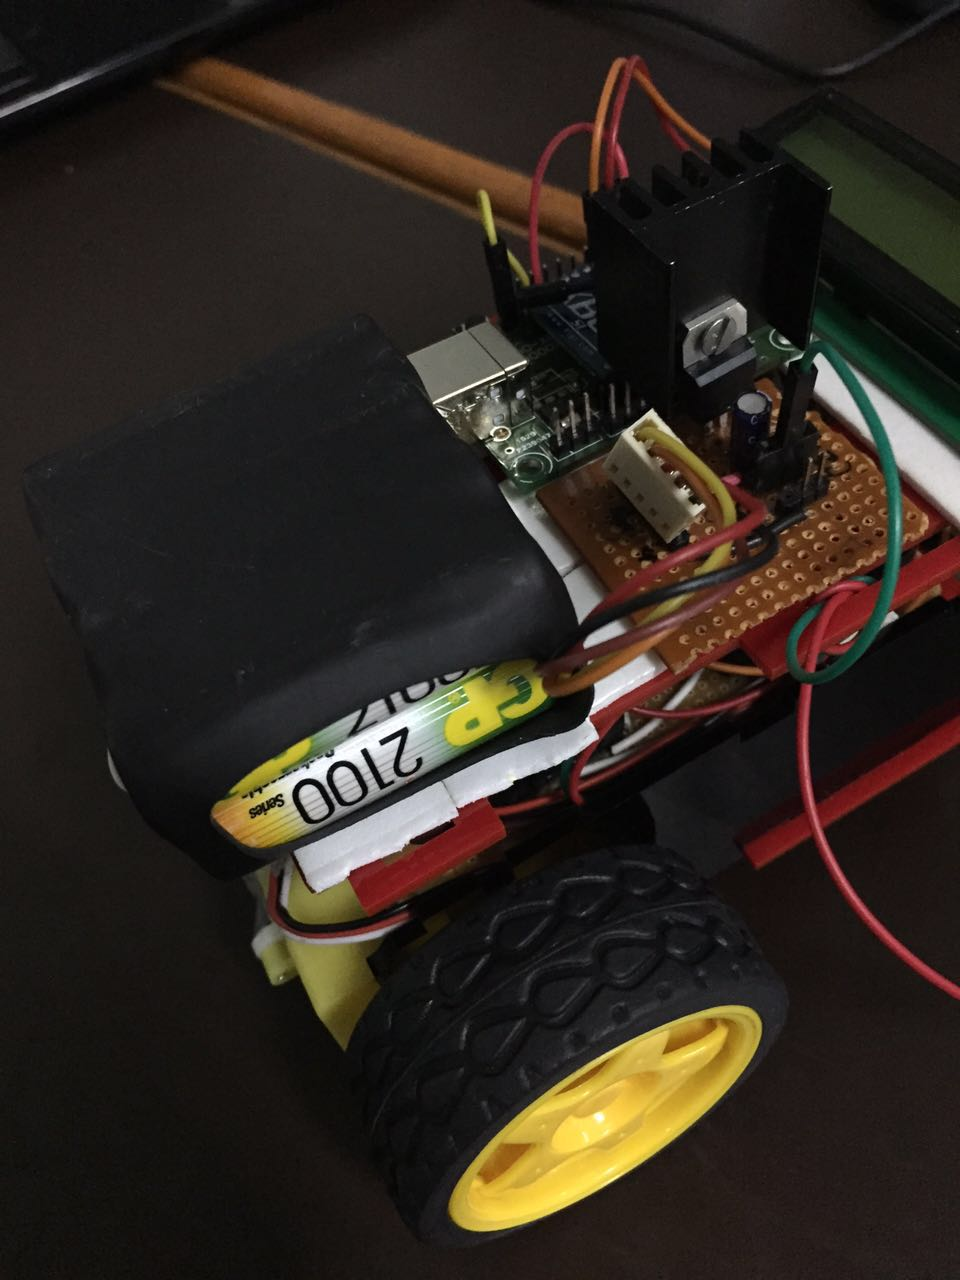
\includegraphics[scale=0.16]{battery_a}
        \caption{ Voltage Regulator Circuit and Battery  after being attached to the Robot}
      \end{figure}

\item Now all the Components are attached to the Robot.
\begin{figure}[h]
        \centering
        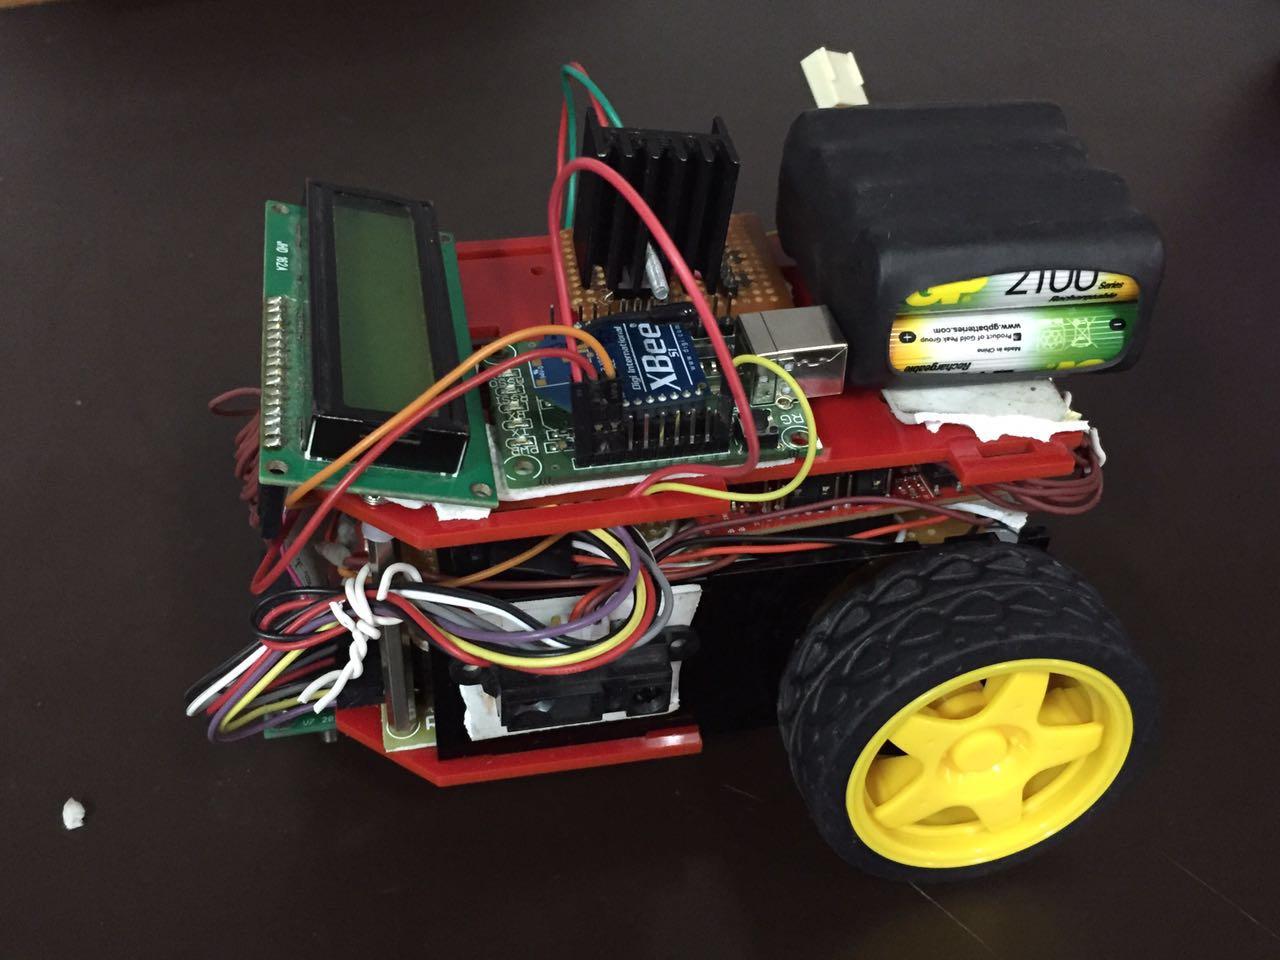
\includegraphics[scale=0.16]{robot}
        \caption{Tiva Robot.}
      \end{figure}
    \newpage
\end{enumerate}

\newpage
\section{Software and Code}
The Github repository can be found at 
 \href{https://github.com/eYSIP-2016/Robot_State_Collector/tree/master/code}{this link}. 
\subsection{State Collection Algorithm}
We use a specific Timer to generate an interrupt after 0.5s. Whenever the interrupt occurs, the state information(i.e. values of all sensors etc.) is collected and transmitted wirelessly to the PC/Laptop via XBee.\\
    Our code is entirely inside the provided header file. A simple function call starts the State Collection.\\
\\
The specific timers used by us to collect the state data for different Robots are as follows:
\begin{itemize}
\item For Fire Bird V -- Timer 4
\item For Tiva Robot - Timer0A
\end{itemize}

NOTE: The Timer used by us cannot be used by the user. 

\subsection{Client GUI and Server}

The GUI is capable of reading the incoming data from the XBee module. We use a symmetric key encryption scheme to encrypt the collected state data. The shared key for symmetric key encryption scheme is encrypted using a public key encryption scheme before it is sent by the client to the server. Encrypted state information can be sent to the server if the user wishes.

\newpage

\section{Use and Demo}

\subsection{Steps for merging the State Collection Code with User's Code for Fire Bird V}
\begin{enumerate}

\item Include "state\_collect.h" in User' Code

\item In main after initialising all the devices call the function  "\_init\_devices()"

\end{enumerate}


NOTE : The files included above should be present inside the same folder as that of the User's code.

\subsection{Steps for merging the State Collection Code with User's Code for Tiva Robot}
\begin{enumerate}

\item Include "common\_header.h" in User' Code

\item In main call the function  "start\_collection()".

\end{enumerate}


NOTE : The files included above should be present inside the same folder as that of the User's code.

\subsection{Steps for Using the GUI}
\begin{enumerate}

\item Make sure that the XBee adapter is connected to the laptop.
\item Click on the "Search for available COM ports " button.
\item From the Drop Down Menu select the COM port on which the XBee adapter is connected. Selecting the COM port would establish a connection with the XBee and the "Not connected" would change to "Connected".
\item After the run is complete click on "End of Run" button to indicate the end of the robot's task.
\item If you want to restart your run press on the "Restart Run" button.
\item To send the data to the server click on "Connect to the Server" button.
\item Login with the credentials provided at the time of registration. This automatically sends the data to the server. 
\item To disconnect from the COM port press the "Disconnect" button.

\end{enumerate}

\subsection{Steps for setting up the Server}
\begin{enumerate}
\item The following list of libraries should be included in the project. Paste the .jar files in a new folder named ``lib'' which should be in the same parent directory as the source files.
\begin{itemize}
	\item \href{http://www.java2s.com/Code/JarDownload/apache-commons/apache-commons}{appache-commons}
	\item \href{https://downloads.bouncycastle.org/java/bcprov-ext-jdk15on-154.jar}{bouncycastle}
	\item \href{http://www.java2s.com/Code/JarDownload/rxtx/rxtx-2.1.7.jar.zip}{gnu}
\end{itemize}
\item The code can be compiled using the following command:
\begin{verbatim}
javac -cp ".:./lib/file1.jar:./lib/file2.jar:
		./lib/file3.jar" decp.java 
\end{verbatim}

Replace the file names with the names of downloaded files.
 
\item In the parent folder containing the source file, the files listed below should be present.
	\begin{itemize} 
		\item "keyStoreName.jceks"
	
	\end{itemize} 
\item Start the server by running the java program using the following command:
\begin{verbatim}
java -cp ".:./lib/file1.jar:./lib/file2.jar:
		./lib/file3.jar" decp 
\end{verbatim}
Again replace the file names with the names of downloaded files.

\item To generate a new Private and Public key Pair just run the code within "serial.java". And then just provide the newly generated "publicKey.txt".

\end{enumerate}


\newpage

\section{Future Work}

\begin{enumerate}

\item LCD, Buzzer and Position Encoders data can be collected.
\item Position encoders can be configured with the Tiva Robot.

\end{enumerate}

\newpage

\section{Bug Report and Challenges}

\subsection{Bugs}


\begin{enumerate}

\item XBee doesn't run at baud rate of 115200 on Fire Bird V.
\item XBee doesn't run at baud rate of 9600 on Tiva Robot.
\item If we change the frequency of the system clock on Tiva Robot the XBee doesn't work.
\item If we have to collect data of the position encoders then it has to be done with the interrupt used by the user and hence we have to change the user's code a bit.
\item The server side code hasn't been tested with multiple clients.
\item There would be a loss of data if the user presses the Disconnect button while the GUI is collecting the State data.
\item On Tiva board no formula for conversion of digital values of Sharp sensor to actual distance has been used as Tiva board has a 12 bit ADC channel and all the formulas that were found were meant for 8 bit ADC channels.

\end{enumerate}

\subsection{Challenges}

\begin{enumerate}

\item Storing the Data efficiently on the Robot's memory -- This was avoided by sending the data using a XBee module.
\item We were first transmitting the data as soon as it was read. This caused a problem as the earlier data was not sent and the new data arrived which caused them to overlap and hence resulted in loss of information -- This was solved by waiting for the previous data to be sent first and then sending the new data.
\item Encryption without using any padding as the data size was not a multiple of 16 bytes and hence the AES encryption algorithm would fail -- This was solved by using a padding which ensures that the data is always a multiple of 16 bytes.
\item Sending the data in a integer format using XBee module -- This was solved by digitising the integer and then sending it.
\item Power when provided directly at VBUS of the TM4C123GXL would cause the robot to restart -- The cause of the problem could not be determined. However the problem vanished automatically after two days.
\item Motor Driver IC would not run from the 5V coming from the Tiva board -- The cause of the problem could not be determined. However the problem vanished automatically during testing.
\item The PIN PF0 was locked and we were unaware of this fact and tried using this port like any other pin -- After a lot of research on the web we found how to unlock the pins.

\end{enumerate}


\begin{thebibliography}{li}



\bibitem{Reading data from USART}Reading data from the USART\\
\href{http://extremeelectronics.co.in/avr-tutorials/using-the-usart-of-avr-microcontrollers-reading-and-writing-data/}{Blog Link}

\bibitem{AES}AES,  {\em Advanced Encryption Standard Basic}\\
\href{https://www.youtube.com/watch?v=liKXtikP9F0}{Youtube Video Link}

\bibitem{Byte Padding}Byte Padding, {\em Padding tutorials}\\
\href{https://en.wikipedia.org/wiki/Padding\_(cryptography)#Byte\_padding}{Wikipedia Link}

\bibitem{Crypto and Block Cipher Modes}Cryptography, {\em Crypto and Block Cipher Modes } \\
\href{https://www.youtube.com/watch?v=t0pREiDO7_g}{Youtube Video Link}

\bibitem{serial}
Serial Communication, {\em Serial Communication in Java With Example Program}\\
\href{https://blog.henrypoon.com/blog/2011/01/01/serial-communication-in-java-with-example-program/}{Blog Link}
\bibitem{java}
GUI, {\em GUI to Implement Rx \& Tx Communication With serial Port}\\
\href{https://www.youtube.com/watch?v=hteeNdA7pOo}{Youtube Video Link}

\bibitem{TI}
TI E2E Community, {\em Unlocking of Locked Pins of Tiva.} \\
\href{https://e2e.ti.com/support/microcontrollers/tiva_arm/f/908/t/284566}{Forum link}

\bibitem{TI}
TI E2E Community, {\em Direct Supply to Tiva Board through VBUS.} \\
\href{https://e2e.ti.com/support/microcontrollers/tiva_arm/f/908/t/346725}{Forum link}

\end{thebibliography}


\end{document}

